\chapter{Revisão bibliográfica}\label{cap:revisao}

Esta seção apresenta conceitos e fundamentos teóricos para o desenvolvimento deste trabalho. São apresentados tópicos relacionados a comunicação por satélites, evolução do sistema ARGOS, e técnicas de modulação, codificação e sincronização envolvidas no padrão \gls{PTT-A3}. O objetivo é fornecer uma base de conhecimento para a compreensão dos requisitos técnicos e operacionais do sistema de comunicação proposto.

\section{COLETA DE DADOS SBCDA VIA SATÉLITE }\label{sec:sbcda}

A comunicação por satélites desempenha um papel fundamental na coleta e disseminação de dados ambientais em escala regional e global. No contexto brasileiro, essa função é desempenhada pelo \gls{SBCDA}, operado pelo \gls{INPE}. O \gls{SBCDA} é composto pelos satélites \gls{SCD-1}, \gls{SCD-2} e \gls{CBERS-1} até \gls{CBERS-4} apresentados na \autoref{fig:satelites} abaixo, que orbitam a aproximadamente 750 km de altitude, recebendo informações transmitidas por \gls{PCD} espalhadas pelo território nacional \cite{lima_parallel_2021}.


\begin{figure}[ht]
    \centering
    \caption{Satélites para coleta de dados ambientais}
    \label{fig:satelites}
    \begin{minipage}[t]{0.48\linewidth}
      \centering
      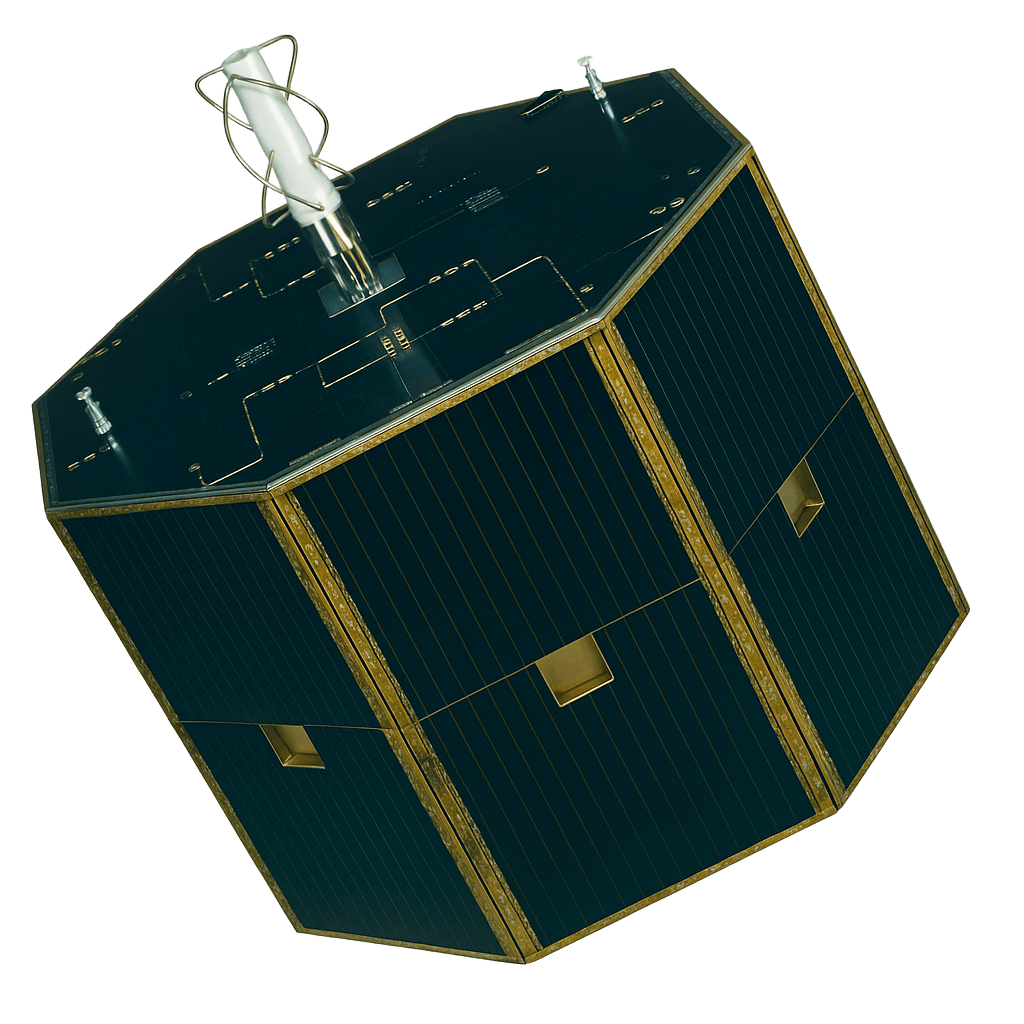
\includegraphics[width=0.7\linewidth]{assets/sat-SCD-1.png}
      \vspace{0.5em}
      \caption*{Satélite SCD-1}
      \small
      \begin{tabularx}{\linewidth}{>{\centering\arraybackslash}X >{\centering\arraybackslash}X}
        \toprule
        \textbf{Parâmetro} & \textbf{Valor} \\
        \midrule
        Massa & 115 kg \\
        Potência Elétrica & 110 W \\
        Vida útil & 4 anos \\
        Altitude média & $\approx$ 750 km \\
        Inclinação orbital & 25$^\circ$ \\
        Período orbital & 99,7 min \\
        \bottomrule
      \end{tabularx}
    \end{minipage}
    \hfill
    \begin{minipage}[t]{0.48\linewidth}
      \centering
      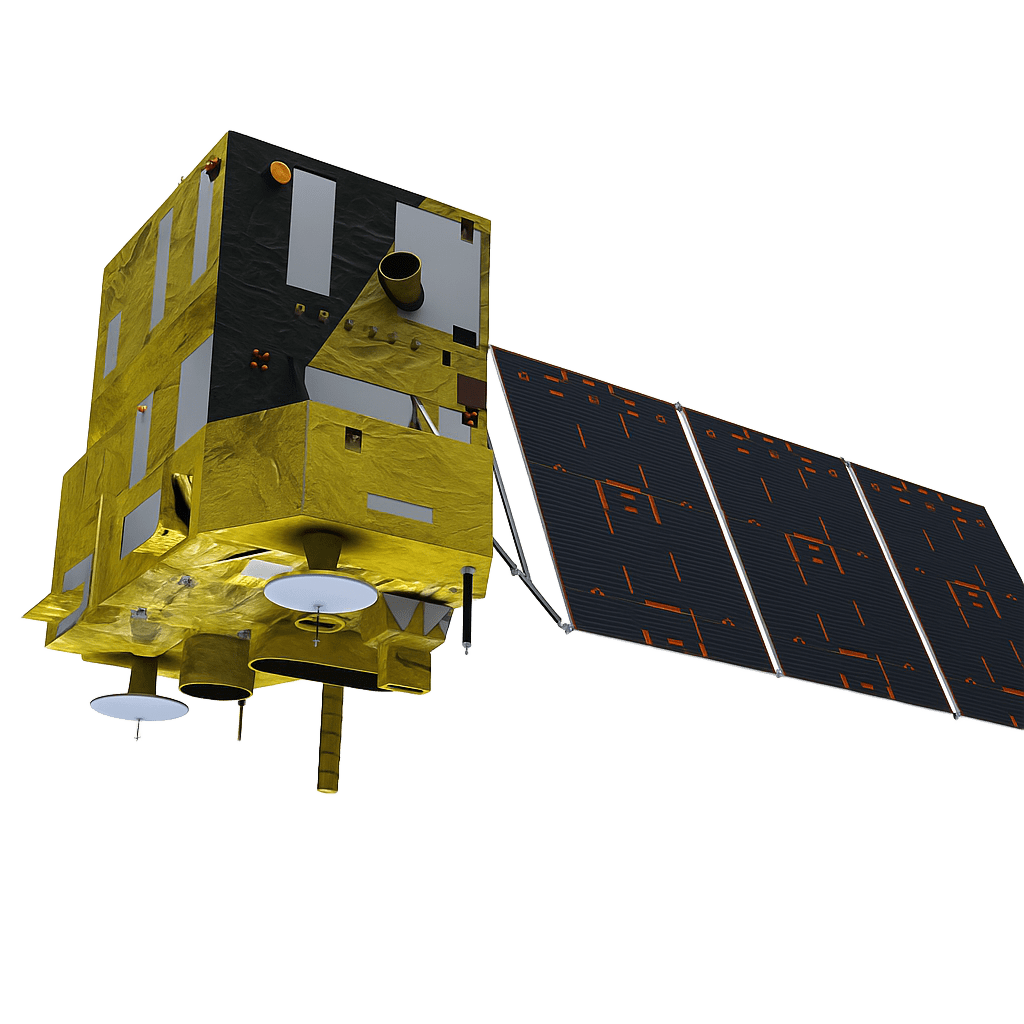
\includegraphics[width=0.7\linewidth]{assets/sat-CBERS-4.png}
      \vspace{0.5em}
      \caption*{Satélite CBERS-4}
      \small
      \begin{tabularx}{\linewidth}{>{\centering\arraybackslash}X >{\centering\arraybackslash}X}
        \toprule
        \textbf{Parâmetro} & \textbf{Valor} \\
        \midrule
        Massa & 1 980 kg \\
        Potência Elétrica & 2 300 W \\
        Vida útil & 3 anos \\
        Altitude média & $\approx$ 778 km \\
        Inclinação orbital & 98,54$^\circ$ \\
        Período orbital & 100,32 min \\
        \bottomrule
      \end{tabularx}
    \end{minipage}
    \vspace{0.5em}
    
\end{figure}

Esses satélites recebem sinais transmitidos pelas \gls{PCD} na faixa de frequência UHF (401,62 a 401,65 \gls{mhz}) e os retransmitem para as \gls{ETR} localizadas em solo, nas faixas de Banda-S (2267,5 \gls{mhz}). Como operam em órbitas baixas, esses satélites realizam aproximadamente 14 revoluções por dia sobre o território nacional, o que permite ampla cobertura espacial.

Apesar da ampla cobertura, a comunicação com satélites de órbita baixa apresenta um grande desafio técnico, sendo a necessidade de visada simultânea entre a \gls{PCD} transmissora e o satélite, o que limita a janela de transmissão e impõe restrições na coleta contínua de dados. Além disso, o movimento relativo entre a \gls{PCD} e o satélite provoca o chamado efeito Doppler, responsável por deslocamentos na frequência do sinal recebido, podendo atingir até ±79,4 kHz. Esse desvio precisa ser compensado para garantir a correta demodulação do sinal \cite{rae2005detector, rodrigues_demodulador_2018}.

A confiabilidade do enlace também é impactada por fatores como atenuação no espaço livre, ruídos térmicos, e variações atmosféricas. Para compensar esses fatores, são necessárias técnicas específicas de modulação, sincronização, codificação de dados e planejamento de enlace, de modo a garantir a confiabilidade das mensagens transmitidas.

\subsection{Constelação Catarina}

A Constelação Catarina é um projeto nacional baseado no uso de nanossatélites em órbita baixa, para atuar como um novo braço operacional do \gls{SBCDA}. A Constelação Catarina é composta por pequenos satélites integrados com \gls{SDR}, capazes de receber sinais transmitidos pelas \gls{PCD} no padrão \gls{ARGOS-II}, com planos futuros de migração para o padrão \gls{ARGOS-III} \cite{gomes_otimizacao_2024}.

Diferentemente dos satélites tradicionais, os nanosatélites da Constelação Catarina são projetados para realizar a decodificação e o armazenamento dos dados a bordo, o que permite superar a limitação de visada simultânea entre satélite e \gls{ETR}, ampliando a cobertura do sistema \cite{rodrigues_demodulador_2018}.

A arquitetura dos satélites que compõem a constelação é baseada na integração do transceptor \gls{AD9361} com uma \gls{FPGA} da \gls{Zynq-7000}, formando uma plataforma de \gls{SDR} altamente flexível \footnote{https://www.argos-system.org/wp-content/uploads/2023/01/ARTIC-Chipset-AnSem-Info-sheet.pdf}. Essa configuração permite a reconfiguração remota do hardware, o que é especialmente importante para futuras atualizações de protocolo ou migração para novos padrões de comunicação, como o \gls{PTT-A3}.


\section{EVOLUÇÃO DO SISTEMA ARGOS}\label{sec:quadros}

O \gls{ARGOS-II}, base do \gls{SBCDA} desde 1993, utiliza transmissores do tipo \gls{PTT-A2}, baseados em modulação analógica \gls{PM} com codificação Manchester. Essa versão se mostrou eficiente por muitos anos, mas suas limitações logo se tornaram evidentes, especialmente no que diz respeito à robustez frente a ruído, à largura de banda ocupada e à necessidade de visada simultânea entre \gls{PCD} e satélite para a \gls{ETR} \cite{cnes_services_and_message_formats_ed2_rev2_2006}.

A evolução desse sistema levou ao desenvolvimento do \gls{ARGOS-III}, que introduziu novas técnicas digitais de comunicação. Essa nova geração incorporou transmissores do tipo \gls{PTT-A3} e \gls{PTT-ZE}, os quais se destacam pela adoção de modulação \gls{QPSK}, codificação convolucional e embaralhamento de dados, resultando em maior confiabilidade na transmissão e maior eficiência espectral. Além disso, o \gls{ARGOS-III} permite o armazenamento e retransmissão de mensagens a bordo do satélite para a \gls{ETR} \cite{lima_parallel_2021, rodrigues_demodulador_2018}.

\section{ESPECIFICAÇÕES DO PADRÃO PTT-A3}

O transmissor do tipo \gls{PTT-A3} é um dos formatos definidos na terceira geração do sistema \gls{ARGOS}, projetado para oferecer maior robustez na transmissão e maior eficiência na utilização do espectro de frequência. 

A estrutura de um quadro \gls{PTT-A3} é composta por três campos principais, sendo eles: portadora pura, palavra de sincronismo (preâmbulo) e datagrama. Na \autoref{fig:estrutura_quadro}, a estrutura é apresentada de forma detalhada, considerando que a taxa de transmissão \gls{Rb} é de 400 \gls{bps} \textcite{cnes_services_and_message_formats_ed2_rev2_2006}.

\begin{figure}[ht]
	\centering
	\caption{Estrutura do quadro de transmissão ARGOS-3}\label{fig:estrutura_quadro}
	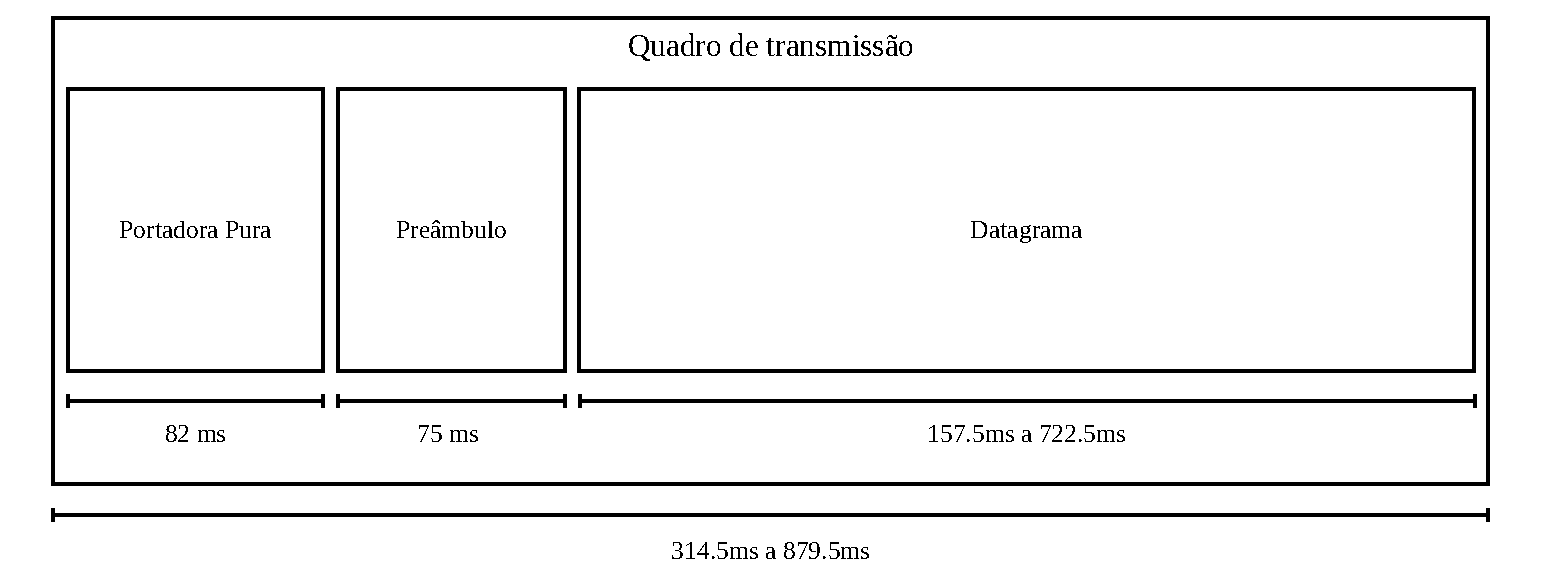
\includegraphics[width=\linewidth]{assets/quadro.pdf}
\end{figure}

\subsection{Portadora pura}

A sequência de transmissão do quadro inicia-se com a portadora contínua ou pura, com duração de 82 ± 2 ms. Durante essa etapa a portadora não transmite dados modulados e é utilizada pelo receptor apenas para realizar a detecção do sinal, bem como para facilitar o processo de sincronização de frequência e fase da portadora. 

A \autoref{fig:portadora_pura_freq} apresenta o sinal da portadora pura no espectro em comparação com o sinal modulado. Nota-se que quando apenas a portadora pura é transmitida, o espectro do sinal é concentrado em uma única frequência, sem componentes laterais. Já o sinal modulado apresenta componentes laterais que se estendem ao redor da frequência da portadora \gls{fc}, formando uma banda de uso do espectro mais ampla \cite{cnes_services_and_message_formats_ed2_rev2_2006}.


\begin{figure}[ht]
	\centering
	\caption{Simulação de portadora pura no domínio da frequência}\label{fig:portadora_pura_freq}
	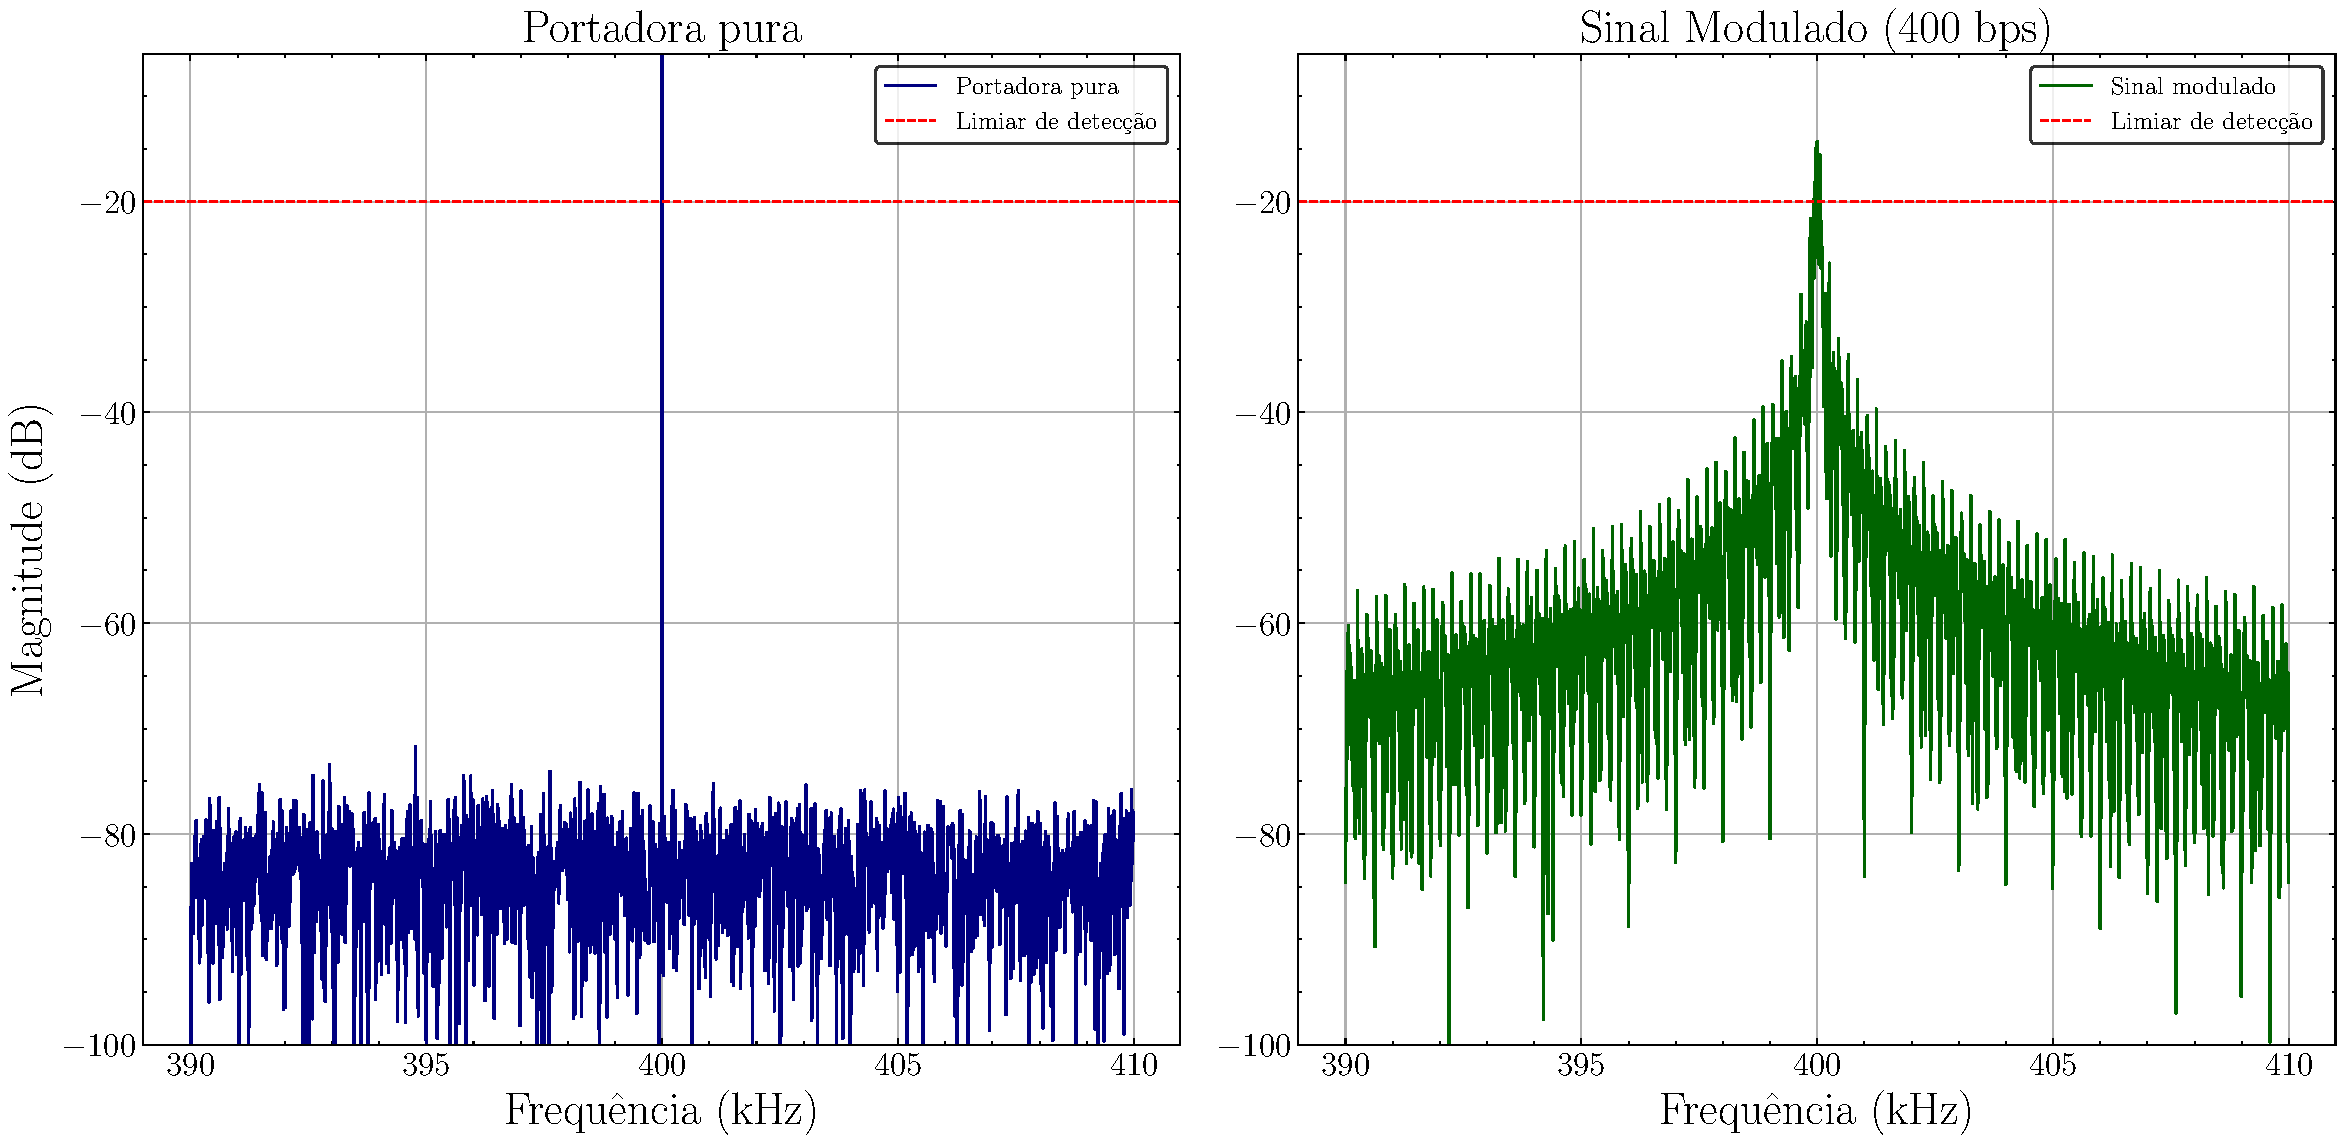
\includegraphics[width=\linewidth]{assets/plots/carrier_spectra.pdf}
    
\end{figure}

O processo de detecção do sinal realizado pelo receptor monitora a presença de sinal que ultrapassa um determinado limiar, dessa forma é fundamental que no receptor o sinal esteja o mais concentrado e com a maior \gls{SNR} possível no momento da detecção, para que a frequência da portadora, \gls{fc}, seja identificada corretamente \cite{cnes_services_and_message_formats_ed2_rev2_2006}.


\subsection{Palavra de sincronismo}

Logo após a portadora pura, é transmitida uma palavra de sincronismo de 30 bits (correspondente a 15 símbolos \gls{QPSK}), cuja função é auxiliar na identificação do início da mensagem codificada, possibilitando a sincronização para decisão. Essa sequência é conhecida e fixa entre transmissor e receptor, no caso do \gls{PTT-A3} sendo $S = \text{2BEEEEBF}_{16}$, o que permite alinhar corretamente a decisão e identificar o início do bloco de dados úteis. \cite{cnes_services_and_message_formats_ed2_rev2_2006}

A sequência \gls{Sn} é separada em dois vetores distintos, \gls{SIn} e \gls{SQn}, por meio de uma intercalação simples de seus bits. O processo de intercalação consiste em distribuir os bits de forma alternada entre os canais \gls{SIn} e \gls{SQn}, resultando em duas sequências de 15 bits cada, que serão transmitida como preâmbulo \cite{cnes_services_and_message_formats_ed2_rev2_2006}, usando a sequência padrão do \gls{ARGOS-III} podemos representar como

\vspace{-1em}
\begin{equation}
\begin{aligned}
    S_I[n] &= [S_0,\ S_2,\ S_4,\ \dots,\ S_{28}] &\mapsto&  S_I[n] = [1111,\ 1111,\ 1111,\ 111]     \\
    S_Q[n] &= [S_1,\ S_3,\ S_5,\ \dots,\ S_{29}] &\mapsto&  S_Q[n] = [0011,\ 0101,\ 0100,\ 111]
\end{aligned}
\label{eq:intercalacao}
\end{equation}

\noindent Importante destacar que esta palavra não é codificada convolucionalmente ou embaralhada, sendo adicionada ao início do vetor de bits de cada canal após esses blocos.  \cite{cnes_services_and_message_formats_ed2_rev2_2006}. 
